\documentclass[12pt,titlepage,bibliography=totoc]{article}
\usepackage[utf8]{inputenc}
\usepackage[T1]{fontenc}
\usepackage[english]{babel}
\usepackage[a4paper]{geometry}
\frenchspacing
\usepackage{amsfonts}
\usepackage{amsmath}
\usepackage{amssymb}
\usepackage{amsthm}
\usepackage{setspace}
\usepackage{fullpage}
\usepackage{tocbibind}
\usepackage{graphicx}
\usepackage{url}
\usepackage{verbatim}
\usepackage{listings}
%\usepackage{gitinfo2}
\usepackage{hyperref}
\usepackage{cleveref}
\usepackage{cite}
\usepackage{color}
\usepackage{enumitem}
\usepackage{usecases}
\usepackage{nameref}

\definecolor{pblue}{rgb}{0.13,0.13,1}
\definecolor{pgreen}{rgb}{0,0.5,0}
\definecolor{pred}{rgb}{0.9,0,0}
\definecolor{pgrey}{rgb}{0.46,0.45,0.48}
\lstset{language=Java,
  showspaces=false,
  showtabs=false,
  breaklines=true,
  showstringspaces=false,
  breakatwhitespace=true,
  commentstyle=\color{pgreen},
  keywordstyle=\color{pblue},
  stringstyle=\color{pred},
  basicstyle=\ttfamily,
  moredelim=[il][\textcolor{pgrey}]{$$},
  moredelim=[is][\textcolor{pgrey}]{\%\%}{\%\%}
}
\renewcommand{\labelitemi}{$\bullet$}
\renewcommand{\labelitemii}{$\cdot$}
\renewcommand{\labelitemiii}{$\diamond$}
\renewcommand{\labelitemiv}{$\ast$}


\begin{document}
\title{
	Design Document for Bicycle Garage Pro\\
	(Group 33, 2015)\\
	\vspace{0.2in}
	\normalsize Current version: 0.9.1
}
\author{
	Alexander Skafte\\
	\url{tfy13ask@student.lu.se}\\
	Dennis Jin\\
	\url{desuvader@gmail.com}\\
	Petter Berntsson\\
	\url{dat14pbe@student.lu.se}\\
	Emelie Löthman\\
	\url{pol14elo@student.lu.se}\\
	Adam Mzrozek\\
	\url{dat14amr@student.lu.se}
}
\date{}



\maketitle
\newpage
\tableofcontents
\thispagestyle{empty}
\setcounter{page}{0}
\newpage

\section{Introduction}
\subsection{References}
\subsection{Purpose}
This document describes the requirements and functionalities of the "Bicycle Garage Pro" (BGP) software.

The intended audience of this document are mainly: software developers, in order to aid the development of the software; and clients, in order to provide an accurate overview of the project.

\subsection{Glossary}
Despite this being a software-only specification, relevant hardware-related terms are still mentioned for convenience sake.
\begin{enumerate}
	\item General terms
	\begin{enumerate}
		\item BGP - Bicycle Garage Pro (software)
		\item ACME - The company which BGP is produced for
		\item User - Cyclist who uses the Bicycle Garage Pro system
		\item Operator - Subject responsible for managing BGP (on-site)
		\item Entrance - Main entrance door of the garage
		\item Exit 1 - Garage exit for users with bicycles
		\item Exit 2 - Garage exit for users without bicycles
	\end{enumerate}

	\item Software-related terms
	\begin{enumerate}
		\item (The) System - Bicycle Garage Pro software
		\item PIN - Four-digit code, used to access the garage
		\item API - Application programming interface
	\end{enumerate}

	\item Hardware-related terms
	\begin{enumerate}
		\item LED - Light-emitting diode
		\item Barcode reader - Device that can read/scan barcodes
		\item Barcode printer - Device that can print barcodes
		\item PIN terminal - Terminal where a PIN can be entered
		\item Electronic lock - Electronically controlled lock on the entrance and exit 1
	\end{enumerate}
\end{enumerate}

\subsection{Scope}
BGP is a software application that manages a bicycle garage. This requirement specification only covers the software part for the bicycle garage and the following assumptions are therefore made about the hardware:
\begin{enumerate}
	\item The hardware handles recognition and reading (scanning) of barcodes
	\item The hardware handles printing of barcodes
	\item The hardware handles locking and unlocking of doors
	\item The hardware handles reading of PINs
\end{enumerate}
The hardware, as stated above, will be accessed by the system according to a predefined API. See \cref{app:hardware} for a more detailed description of the API.

\subsection{Goals}
\subsubsection{Business goals}
ACME is a company that works in the bicycle garage business. ACME aims to provide low-cost, semi-automated bicycle garage solutions for public use. The goals for ACME with this software are mainly:
\begin{enumerate}
	\item Customer retention through maintainability
\end{enumerate}
\subsubsection{Product goals}
The goal of BGP is to assist in managing a bicycle garage by keeping track of users and their bicycles. The user interface should be simple to use and the software should be easily maintainable for future developers.

\subsection{Overview}
The structure of this specification is based on guidelines from the ETSA01 course website and the ETSA01 course compendium \cite{kompendium,course-site}.

\section{Product description}
\begin{figure}
	\centering
	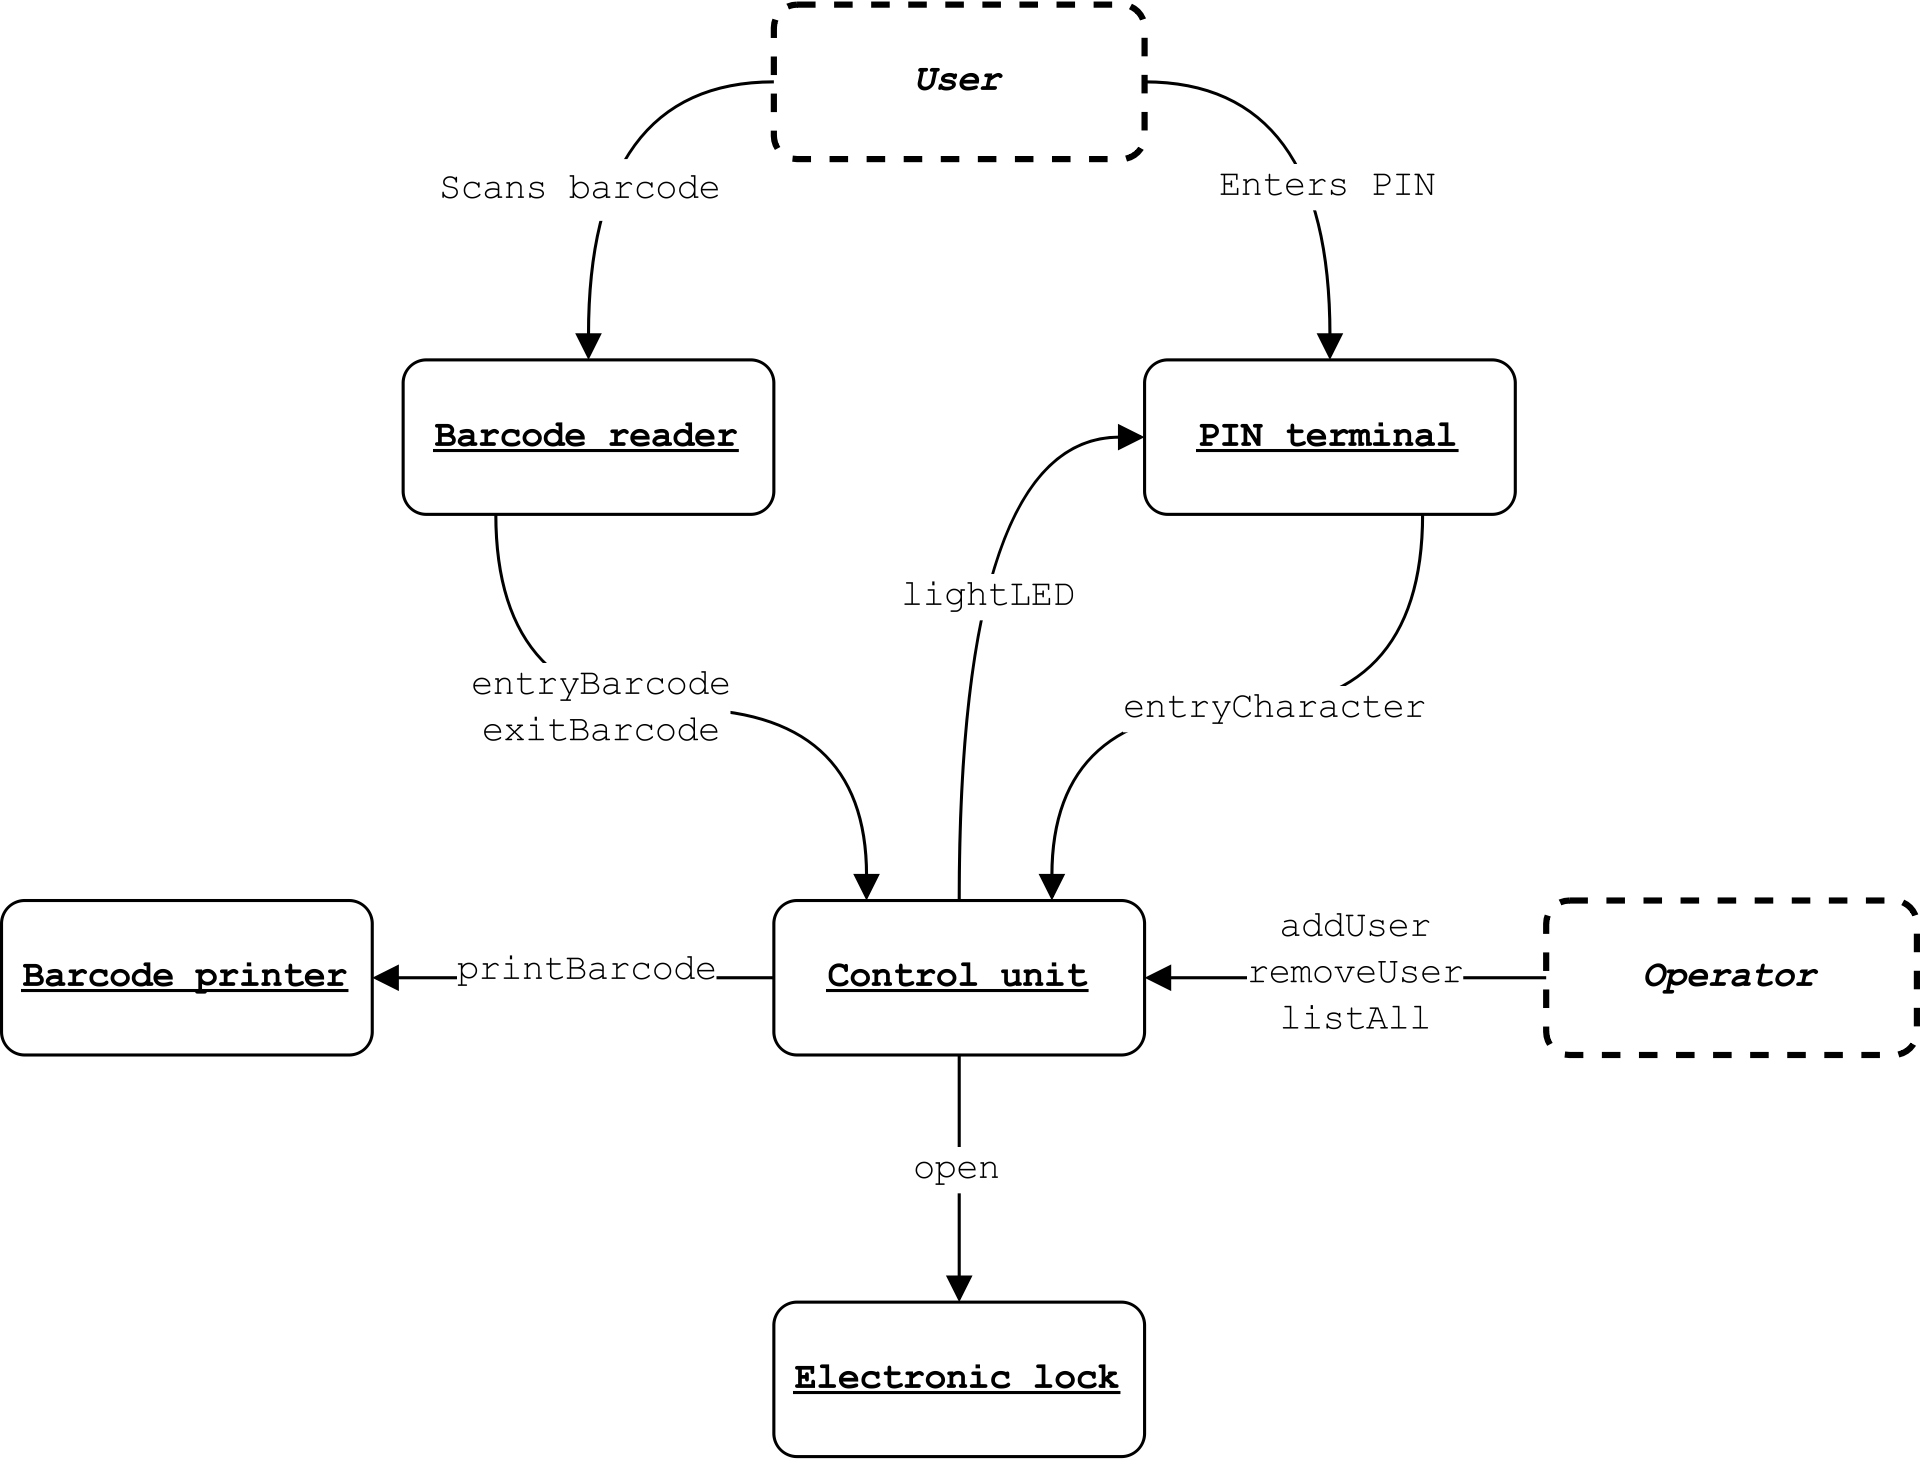
\includegraphics[width=0.9\textwidth]{./assets/context-hw-nobox.png}
	\caption{Context diagram for BGP}
	\label{fig:context-hw}
\end{figure}

The interactions between the system and external entities, that may interact with the system, can be seen in \cref{fig:context-hw}. The control unit is the BGP software. The arrows mainly aim to specify software-related signals that are relevant to this specification.

\begin{enumerate}
	\item The control unit sends out the following signals:
	\begin{enumerate}
		\item lightLED - Sent out depending on success/failure when entering PIN or scanning barcode
		\item printBarcode - Sent out when a barcode should be printed through the barcode printer
		\item open - Sent out to either the entrance or exit 1, and unlocks the door (electronic lock)
	\end{enumerate}
	\item The control unit receives the following signals:
	\begin{enumerate}
		\item entryCharacter - Received when a button is pressed on the PIN terminal
		\item entryBarcode - Received when a barcode is scanned at the entrance
		\item exitBarcode - Received when a barcode is scanned at the exit
		\item addUser - Received when the operator wants to add an user
		\item removeUser - Received when the operator wants to remove an user
		\item searchUser - Received when the operator wants to search for an user
	\end{enumerate}
\end{enumerate}

\section{Requirements}



\bibliography{bibliography}{}
\bibliographystyle{plain}
\appendix

\section{Hardware API}
\label{app:hardware}
This API specification is directly copied from \url{http://cs.lth.se/etsa01/projekt-2015/haardvarugraenssnitt-och-drivrutiner/}. If there are any questions regarding the hardware API, please contact Markus Borg (\url{Markus.Borg@cs.lth.se}).

\begin{lstlisting}[language=Java]
public interface BarcodePrinter {
	/* Print a bicycleID as a barcode.
	 * Bicycle ID should be a string of 5 characters, where every
	 * character can be '0', '1',... '9'. */

	public void printBarcode(String bicycleID);
}

public interface PinCodeTerminal { 
	/* Register bicycle garage manager so 
	 * that the pin code terminal knows 
	 * which manager to call when a user has 
	 * pressed a key. */ 

	public void register(BicycleGarageManager manager); 

	/* Turn on LED for lightTime seconds. 
	 * Colour: 
	 * colour = RED_LED = 0 => red 
	 * colour = GREEN_LED = 1 => green */ 

	public void lightLED(int colour, int lightTime); 
	public static final int RED_LED = 0, 
	GREEN_LED = 1;
}

public interface BarcodeReader {     
	/* Register bicycle garage manager 
	 * so that the bar code reader knows 
	 * which manager to call when a user 
	 * has used the reader. */  

	public void register(BicycleGarageManager manager); 
}

public interface ElectronicLock {
	/* Open the lock for timeOpen seconds.  */

	public void open(int timeOpen);
}
\end{lstlisting}
\end{document}